\documentclass{beamer}
\usecolortheme{default}
\usepackage{graphics}
\usepackage{karnaugh-map}
\usepackage{tikz}
\usetikzlibrary{circuits.logic.US,calc}
\usetheme{Boadilla}
\usebackgroundtemplate{\includegraphics[width=\paperwidth,height=\paperheight]{Screenshot_2021-01-09-17-07-10-10.jpg}}

\title{Presentation}
\author{Sikander Kathat}
\institute{IIIT Raichur}
\date{8 january 2021}
\begin{document}

<presentation>


\titlepage here is my presentation starts:
 \section{Section 1}
\subsection{sub a}

\begin{frame}
\frametitle{Question statement:}

A 4:1 multiplexer is to be used for generating the output carry of a full adder. A and B are the bits to be added while $C_{in}$ is the input carry and $C_{out}$ is the output carry. A and B are to be used as select bits with A being more significant select bit.

Which one of the following statement correctly describes the choice of signals to be connected to the inputs  $ I_0, I_1, I_2 and I_3 $  so that the output is $C_{out}$  ?
\end{frame}

\begin{frame}
\frametitle{options}
\begin{enumerate}
    \item$I_0=0,  I_1=C_i_n,  I_2=C_i_n,  I_3=1$
    \item$I_0=1,  I_1=C_i_n,  I_2=C_i_n,  I_3=1$
    \item$I_0=C_i_n,  I_1=0,  I_2=1,  I_3=C_i_n$
    \item$I_0=0,  I_1=C_i_n,  I_2=1,  I_3=C_i_n$
\end{enumerate}
    
\end{frame}
 
 \begin{frame}
\frametitle{ANSWER:-}
 $I_0=0,  I_1=C_i_n,  I_2=C_i_n,  I_3=1$
 
 \end{frame}
 
  \begin{frame}
\frametitle{MUX Diagram}
 \begin{figure}[!ht]
\centering
{
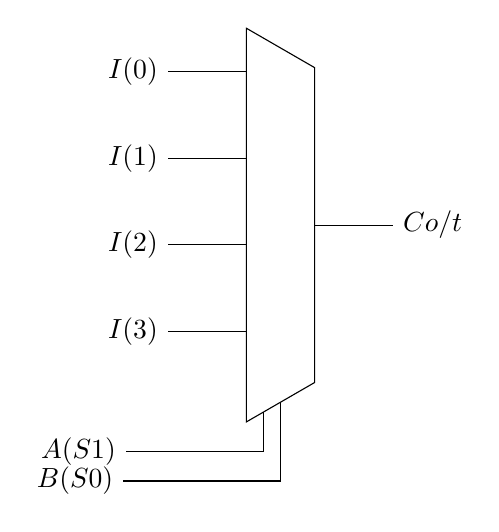
\begin{tikzpicture}
\draw (0,0)coordinate (O)--++(30:1)coordinate (P)--++(90:4)coordinate (Q)--++(150:1)coordinate (R)--cycle;
\draw($(P)!0.5!(Q)$)--++(0:1)node[right]{$Co/t$};
\draw($(O)!0.5!(P)$)--++(-90:1)--++(180:2)node[left]{$B(S0)$};
\draw($(O)!0.25!(P)$)--++(-90:0.5)--++(180:1.75)node[left]{$A(S1)$};
\foreach\y/\t in {0.1/(0),0.3/(1),0.5/(2),0.7/(3)} {
\draw ($(R)!\y*1.1!(O)$)--++(180:1)node[left]{$I\t$};}
\end{tikzpicture}

}
\caption{question MUX diagram}
\label{MUX diagram)}
\end{figure}
\end{frame}
 
   \begin{frame}
\frametitle{Solution}
\framesubtitle{TRUTH TABLE}
  \begin{table}[!ht]
\centering
{
\begin{tabular}{|l|l|l|l|l|}
\hline
A & B & C(in) & Sum(S) & Co/t \\ \hline
0 & 0 & 0     & 0      & 0    \\
0 & 0 & 1     & 1      & 0    \\
0 & 1 & 0     & 1      & 0    \\ 
0 & 1 & 1     & 0      & 1    \\
1 & 0 & 0     & 1      & 0    \\
1 & 0 & 1     & 0      & 1    \\
1 & 1 & 0     & 0      & 1    \\
1 & 1 & 1     & 1      & 1    \\ \hline
\end{tabular}

}
\caption{TRUTH TABLE}
\label{table}
\end{table}
  \end{frame}
  
 \begin{frame}
\frametitle{Explanation:}  
\begin{figure}[!ht]
\centering
{
\begin{karnaugh-map}[4][2][1][][]
    \maxterms{0,3,5,6}
    \minterms{1,2,4,7}
    \implicant{1}{1}
    \implicant{2}{2}
    \implicant{4}{4}
    \implicant{7}{7}
    % note: position for start of \draw is (0, Y) where Y is
    % the Y size(number of cells high) in this case Y=2
    \draw[color=black, ultra thin] (0, 2) --
    node [pos=1, above right, anchor=south west] {$BC(in)$} % YOU CAN CHANGE NAME OF VAR HERE, THE $X$ IS USED FOR ITALICS
    node [pos=1, below left, anchor=north east] {$A$} % SAME FOR THIS
    ++(135:1);
        
    \end{karnaugh-map}

}
\caption{k-map for Sum}
\label{kmap Sum}
\end{figure}


    
    Boolean expression for Sum  -
    
    
    Sum=A$\overline{B}$ $\overline{C_i_n}$ + $\overline{A}$ $\overline{B}$C_i_n$ + $\overline{A}$ B $\overline{C_i_n}$ + AB$C_i_n$
    
\end{frame}
\begin{frame}
\frametitle{Explanation}

\begin{figure}[!ht]
\centering
{
\begin{karnaugh-map}[4][2][1][][]
    \maxterms{0,1,2,4}
    \minterms{3,5,6,7}
    \implicant{3}{7}
    \implicant{5}{7}
    \implicant{7}{6}
    % note: position for start of \draw is (0, Y) where Y is
    % the Y size(number of cells high) in this case Y=2
    \draw[color=black, ultra thin] (0, 2) --
    node [pos=1, above right, anchor=south west] {$BC(in)$} % YOU CAN CHANGE NAME OF VAR HERE, THE $X$ IS USED FOR ITALICS
    node [pos=1, below left, anchor=north east] {$A$} % SAME FOR THIS
    ++(135:1);
        
    \end{karnaugh-map}

}
\caption{k-map for $C_o_u_t$}
\label{kmap $C_o_u_t$}
\end{figure}
 
 Boolean expression for $C_o_u_t$  -

$C_o_u_t$= B$C_i_n$ + AB + A$C_i_n$

\end{frame}
\begin{frame}
\frametitle{Explanation:}
    
\begin{table}[!ht]
\centering
{
\begin{tabular}{|l|l|l|} \hline
A & B & C o/t  \\ \hline
0 & 0 & 0      \\
0 & 1 & C(in)  \\
1 & 0 & C(in)  \\
1 & 1 & 1      \\ \hline
\end{tabular}



}
\caption{TRUTH TABLE for $C_o_u_t$ to be output}
\label{table 1 }
\end{table}

So, our final answer is=

$I_0=0,  I_1=C_i_n,  I_2=C_i_n,  I_3=1$
  
   \end{frame}
   
   \begin{frame} 
   \frametitle{COMPLETE}
	    
	    \centering THANK YOU
	    
	   \end{frame}  
	    
\end{document}